\documentclass[8pt, twosided, a4paper]{article}
% 8 point font, A4-sized paper

\usepackage[margin=2.5cm]{geometry}
\usepackage[utf8]{inputenc}

\usepackage[scaled]{helvet}
\renewcommand\familydefault{\sfdefault} 
\usepackage[T1]{fontenc}

\usepackage{pdfpages}
\usepackage{subfiles}
\usepackage{setspace}
\usepackage{multicol}
\usepackage{multirow}
\usepackage{mathtools}

\usepackage{cancel}

\usepackage[inline]{asymptote}

\usepackage{array}
\usepackage{enumitem}
\usepackage{float}
\usepackage{amsfonts}
\usepackage{tikz}
\usetikzlibrary{matrix,fit,tikzmark,calc}
\usepackage{blkarray}
\usepackage{caption}
\usepackage{wrapfig}
\usepackage{hhline}

\newcommand{\twomat}[4] {\left[\begin{array}{cc} #1 & #2 \\ #3 & #4 \end{array}\right]}
\newcommand{\threemat}[9] {\left[\begin{array}{ccc} #1 & #2 & #3 \\ #4 & #5 & #6 \\ #7 & #8 & #9 \end{array}\right]}

\newcommand{\twovec}[2] {\left[\begin{array}{c} #1 \\ #2 \end{array}\right]}
\newcommand{\stwovec}[2] {\left[\begin{smallmatrix} #1 \\ #2 \end{smallmatrix}\right]}

\newcounter{problem_i}
\newcounter{problem_ii}

\begin{document}
\pagenumbering{gobble}

% I did this because it was too dense without it
\setlength{\parskip}{1em}

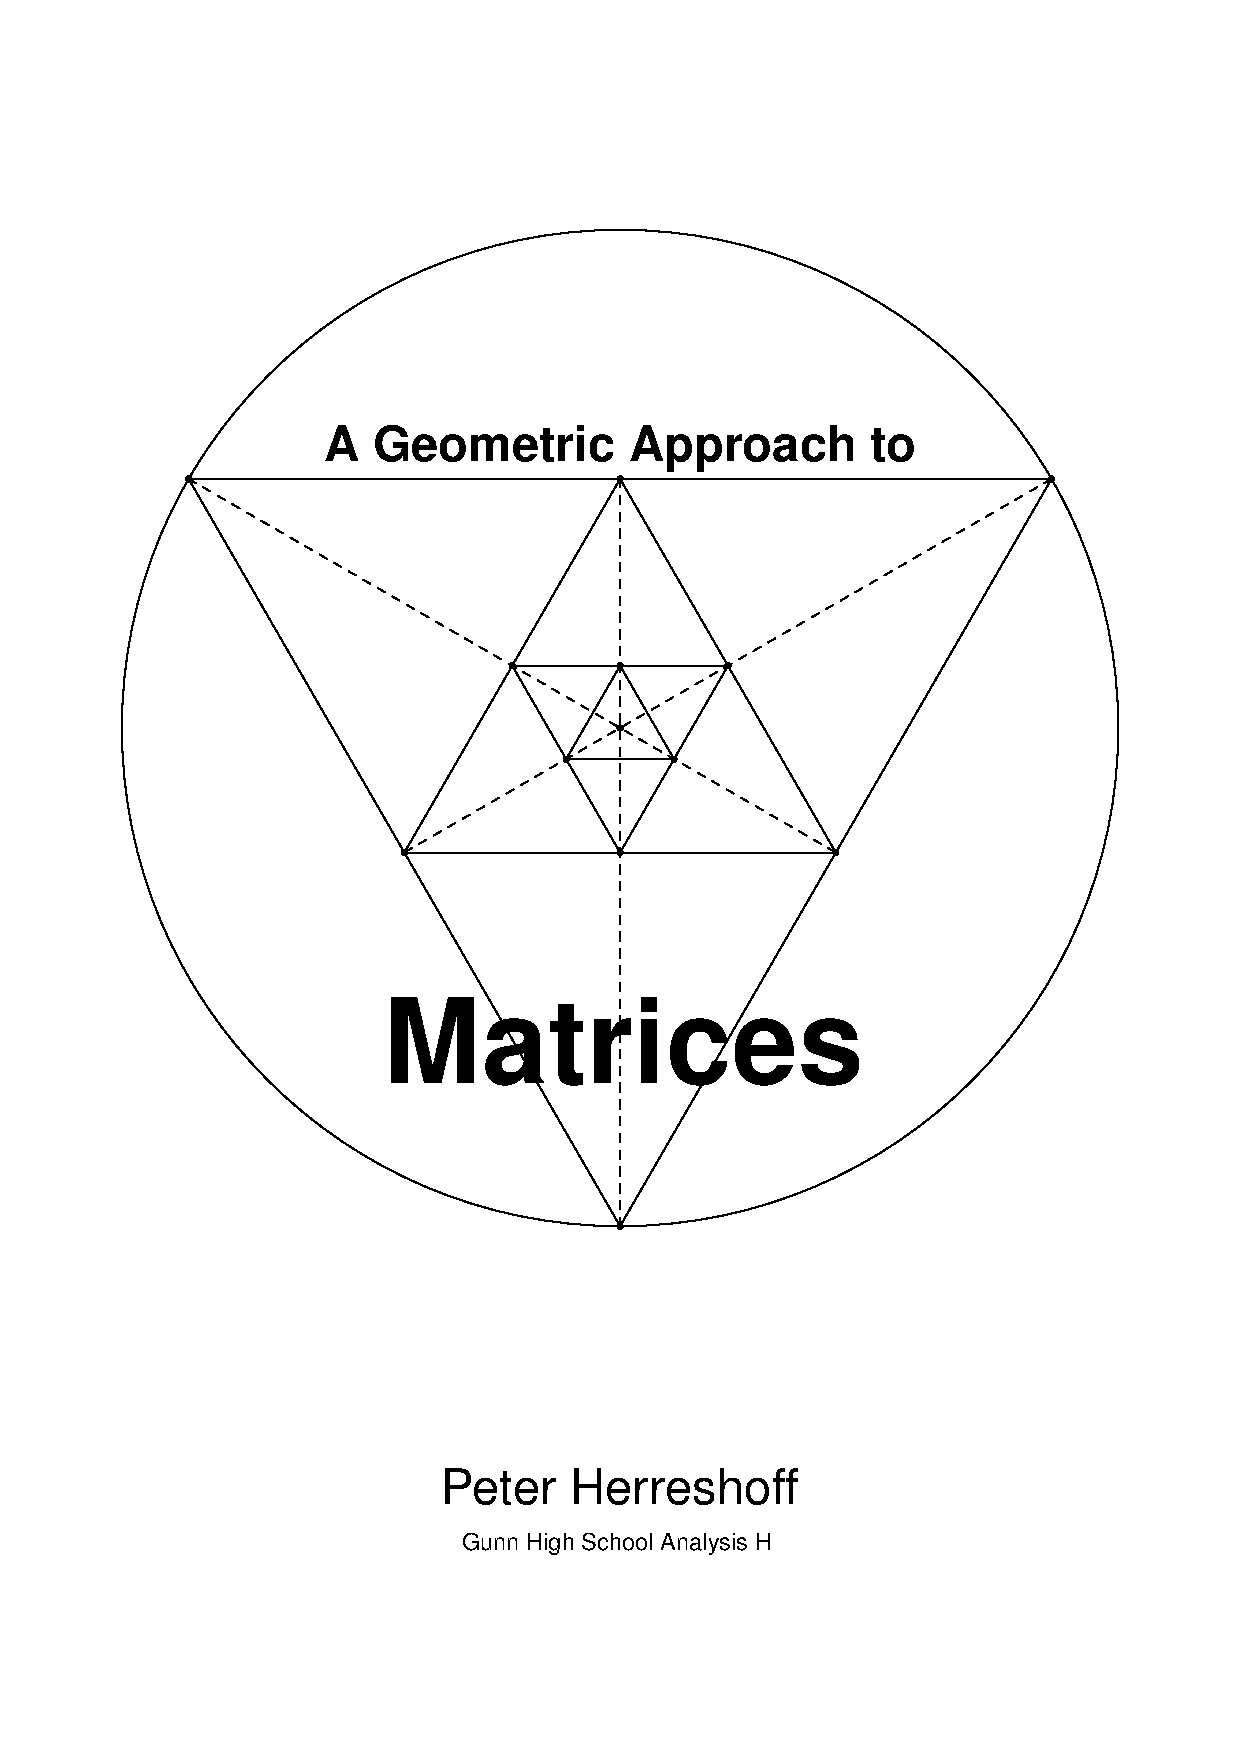
\includepdf[noautoscale=true,pages=-,width=\paperwidth]{./cover/cover_source.pdf} % cover

\subfile{credits/credits_source.tex}
\setcounter{page}{0}
\pagebreak
\pagenumbering{arabic}

\restoregeometry % Because the credits have a different margin setting

\setlength{\parskip}{0.5em}

\tableofcontents
\pagebreak

% Reset to correct value
\setlength{\parskip}{0em}

\subfile{trig_review/trig_review_source.tex} % trig review
\pagebreak

\subfile{itsasnap/itsasnap_source.tex}
\pagebreak

\subfile{snap_flip/snap_flip_source.tex}
\pagebreak

\subfile{rrg/rrg_source.tex} % Rotation reflection groups
\pagebreak

\subfile{inf/inf_source.tex} % Infinite groups
\pagebreak

\subfile{cmplx_geo/cmplx_geo_source.tex} % Geometry of complex numbers
\pagebreak

\subfile{vitamin_i/vitamin_i_source.tex} % Vitamin i
\pagebreak

\subfile{mtrx_mult/mtrx_mult_source.tex} % Matrix multiplication
\pagebreak

\subfile{map_plane/map_plane_source.tex} % Mapping the Plane
\pagebreak

\subfile{plane_rot/plane_rot_source.tex} % Plane rotate
\pagebreak

\subfile{mat_gen/mat_gen_source.tex} % Matrices generate groups
\pagebreak

\subfile{comp_map/comp_map_source.tex} % Composite mappings (fat one)
\pagebreak

\subfile{inverses/inverses_source.tex} % Composite mappings (fat one)
\pagebreak

\subfile{mod_m/mod_m_source.tex} % Modulo m meets groups
\pagebreak

\subfile{eigen/eigen_source.tex} % eigenvectors and eigenvalues
\pagebreak

\subfile{comp_func/comp_func_source.tex} % Composition of functions
\pagebreak

\end{document}